
\section{Analisi dei dati di probabilit\`a}
\label{Analisi dei dati}

\subsection{Problema in esame}
\label{Problema in esame}

Test, sottoposto ad un candidato  durante un colloquio, composto da \textit{domande a tripla risposta multipla}.\\\\ Nel suddetto  documento vengono analizzate le relazioni che intercorrono tra due domande, denominate A e B, a seconda se il candidato risulta in grado di rispondervi correttamente o meno.

\subsection{Caratteristiche degli eventi di coppia}
\label{Caratteristiche degli eventi di coppia}

Tipi di eventi trattati:
\begin{itemize}
\item \textbf{Eventi indipendenti};
\item \textbf{Eventi dipendenti}:
  \begin{itemize}
  \item A e B sono strettamente dipendenti;
  \item A implica B.
  \end{itemize}
\item \textbf{Evento conosciuto ed evento indovinato}.
\end{itemize}
\noindent
Struttura usata per rappresentare la probabilit\`a degli eventi di coppia:

\begin{center}$AB$\end{center}
\begin{center} /\textbackslash \end{center}
\begin{center}$A$   $B$ \end{center}
\begin{center} \textbackslash / \end{center}
\begin{center}$Z$\end{center}
con:

\begin{itemize}
\item \textit{AB} rappresenta la probabilit\`a complessiva dell'evento che si verifica sempre;
\item \textit{A} rappresenta  la probabilit\`a che permette il verificarsi di A, ma non di B;
\item \textit{B} rappresenta la probabilit\`a che permette il verificarsi di B, ma non di A;
\item \textit{Z} rappresenta la probabilit\`a a zero, l'impossibilit\`a del verificarsi dell'evento.
\end{itemize}
\noindent
\subsubsection{Eventi indipendenti}
\label{Eventi indipendenti}
A e B sono due domande la quali risposte sono completamente scorrelate tra di loro.

\begin{center} $P(A)P(B)$ \end{center}
\begin{center} /\textbackslash \end{center}
\begin{center} $P(A)(1-P(B))$  $(1-P(A))P(B)$ \end{center}
\begin{center} \textbackslash / \end{center}
\begin{center} $(1-P(A))(1-P(B))$ \end{center}

\paragraph{Considerazioni generali}
\label{Considerazioni generali eventi indipendenti}
La probabilit\`a complessiva nel caso di domande indipendenti A e B viene data da $P(A)$ per $P(B)$. \\ Se \`e conosciuta dal candidato la risposta alla domanda A ma non alla domanda B la probabilit\`a di ottenere una risposta corretta \`e $P(A)$, mentre la probabilit\`a di ottenere una risposta non corretta per B vale $1-P(B)$. Il ragionamento duale \`e svolto nel calcolo della probabilit\`a per la riposta corretta alla domanda B ma non ad A.\\
La probabilit\`a  di non ottenere alcuna risposta corretta alle due domande  viene calcolata prendendo in considerazione gli eventi contrari a quelli coinvolti. Dunque per  A la probabilit\`a  che il candidato non conosca la soluzione \`e  $1-P(B)$, dualmente per B la probabilit\`a  \`e $1-P(A)$.

\subsubsection{Eventi dipendenti}
\label{Eventi dipendenti}
\paragraph{A e B sono due domande fortemente correlate tra di loro} se si risponde correttamente ad una delle due domande si risponde correttamente anche all'altra.

\begin{center} $P(A)^2$ \end{center}
\begin{center} /\textbackslash \end{center}
\begin{center} 0 0  \end{center}
\begin{center} \textbackslash / \end{center}
\begin{center}  $(1- P(A))^2$ \end{center}

\paragraph{Considerazioni generali}
\label{Considerazioni generali eventi dipendenti}
La probabilit\`a complessiva nel caso di domande dipendenti A e B viene data da $P(A)$ per $P(B)$; ma $P(A)=P(B)$ dunque $P(A)^2=P(B)^2$. \\ Conseguentemente se il candidato non conosce la risposta alla domanda A non pu\`o conoscere la risposta alla domanda B percui la probabilit\`a di conoscere uno dei due eventi \`e pari a 0.\\ 
In questo caso la probabilit\`a a 0 \`e   $(1- P(A))(1- P(B))=(1- P(A))^2$
essendo che A=B.

\paragraph{A implica B}
\label{A implica B}
Se si sa rispondere alla domanda A di conseguenza si \`e in grado di rispondere anche alla domanda B.\\
Tuttavia non vale il ragionamento opposto, se si sa rispondere alla domanda B non significa che si \`e in grado di rispondere alla domanda A.

\begin{center} $P(A)$ \end{center}
\begin{center} /\textbackslash \end{center}
\begin{center} 0  $P(B)-P(A)$ \end{center}
\begin{center} \textbackslash / \end{center}
\begin{center} $1-P(B)$ \end{center}

\subparagraph{Considerazioni generali}
\label{Considerazioni generali A implica B}
\noindent
 La probabilit\`a complessiva nel caso di domande dipendenti A e B viene data esclusivamente da $P(A)$ in quanto la conoscenza di sia di A che di B \`e  possibile solo se si ha piena conoscenza di A.\\  Dunque la probabilit\`a  che si conosca la risposta alla domanda  A ma non a B  \`e impossibile (pari a 0); mentre se si ha conoscenza della domanda B ma non di A la probabilit\`a si stanzia a $P(B)-P(A)$.\\ 
La probabilit\`a a zero \`e $1-P(B)$ indicatore dell'impossibilit\`a  di avere la risposta corretta per A.

\subsection{Evento conosciuto ed evento indovinato}
\label{Evento conosciuto ed evento indovinato}
Durante un test il candidato deve saper scegliere la risposta, corretta o meno, alla domanda posta. Le variabili che entrano in gioco durante l'esecuzione dell'atto non riguardano esclusivamente la conoscenza personale del singolo.
\\
La probabilit\`a di un evento A \`e data dalla formula:
\begin{center} $P(A)=P(A_{C})+P(A_{I})$\end{center} 
Le variabili in uso sono:
\begin{itemize}
\item $P(A_{C})$: probabilit\`a che il candidato sappia rispondere alla domanda A correttamente per sua conoscenza;
\item $P(A_{I})$: probabilit\`a che il candidato sappia rispondere alla domanda A correttamente indovinando.
\end{itemize}

\noindent
Per quanto appena definito sopra valgono le seguenti propriet\`a:
\begin{enumerate}
\item $P(B_{C}|A_{C})=1$

\item $P(B_{C}|A_{I})=P(B_{C})$ 

\item $P(B_{I}|A_{C})=0$

\item $P(B_{I}|A_{I})=P(B_{I})$ 
\end{enumerate}
\noindent

\subsubsection{Probabilit\`a di rispondere correttamente ad una domanda}
\label{Probabilita di rispondere correttamente ad una domanda}
Variabili coinvolte:
\begin{itemize}
\item $P(A)$: probabilit\`a necessaria perch\`e si verifichi, per la domanda A, che il candidato dia la risposta corretta.  Per la legge dei grandi numeri la frequenza porta alla probabilit\`a.
\item $S_{0}$: insieme dei casi in cui in un domanda non viene scartata alcuna risposta dal dominio delle risposte possibili;
\item $S_{1}$: insieme dei casi in cui in una domanda viene scartata una risposta dal dominio delle risposte possibili;
\item $S_{2}$: insieme dei casi in cui in una domanda vengono scartate due risposte dal dominio delle risposte possibili.
\item $P(I)$:  probabilit\`a di dare la risposta corretta alla domanda A indovinando;
\item $P(C)$: probabilit\`a di dare la risposta corretta alla domanda A per conoscenza.
\end{itemize}

\noindent
Sapendo che $P(I)=P(A)-P(C)$ logicamente vale anche $P(A)=P(I)+P(C)$.\\\\
Se un candidato non \`e in grado scartare alcuna risposta dalla domanda ha 1 possibilit\`a su 3 di, indovinando, dare la risposta corretta. Se un candidato invece risulta in grado di scartare una risposta, sbagliata, alla domanda rimane con 1 possibilit\`a  su 2 di poter dare la risposta corretta. Se invece, caso ottimo, il candidato ha piena conoscenza della domanda posta risulta in grado di scartare due risposte sbagliate lasciando un'unica risposta possibile, quella esatta.
Il ragionamento sopra espresso pu\`o venire espresso con la seguente espressione:

\begin{center}$P(A)=P(S_{0})\frac{1}{3}+P(S_{1})\frac{1}{2}+P(S_{2})$\end{center} 


\noindent
Ora individuiamo quale \`e la probabilit\`a effettiva per un candidato di dare la risposta corretta ad una domanda A. \\

$1=S_{0}+S_{1}+S_{2}$

$S_0=1-S_{1}-S_{2}$ \\

Sostituendo: \\

P(A)= $(1-P(S_1) - P(S_2))\frac{1}{3}+P(S_1)\frac{1}{2}+P(S_2)$

    = $\frac{1}{3}-\frac{1}{3}P(S_1)-\frac{1}{3}P(S_1)+\frac{1}{2}P(S_1)+P(S_2)$
    
    =$\frac{1}{3}+\frac{1}{6}P(S_1)+\frac{2}{3}P(S_2)$
   

\begin{figure}[H]
\centering
	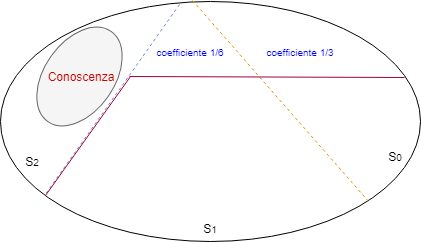
\includegraphics[width=0.60\linewidth]{./image/insieme_probabilita_rispostaesatta.png}
	\caption{Rappresentazione insiemistica della probabilit\`a di rispondere correttamente ad una domanda: P(A)}
\end{figure}
  
  
  
 \paragraph{Considerazioni importanti} \mbox{}\\\\
 \label{Considerazioni importanti}
  In conclusione P(A)=$\frac{1}{3}+\frac{1}{6}P(S_1)+\frac{2}{3}P(S_2)$.
  Ovvero la probabilit\`a  per un candidato di dare in una domanda A la risposta corretta dipende dai seguenti fattori:
  \begin{itemize}
  \item $\frac{1}{3}$: coefficiente che rappresenta la probabilit\`a effettiva per chi non conosce la risposta alla domanda di dare la risposta corretta;
  \item $\frac{1}{2}P(S_1)$: coefficiente che rappresenta la probabilit\`a effettiva di  dare la risposta corretta quando il candidato \`e in grado di scartare una risposta sbagliata alla domanda;
   \item $\frac{2}{3}P(S_2)$: coefficiente che rappresenta la probabilit\`a effettiva di  dare la risposta corretta quando il candidato \`e in grado di scartare due risposte sbagliate alla domanda.
  \end{itemize}
  \noindent
  Dall'analisi della tipologia di eventi di coppia e dal calcolo della probabilit\`a necessaria per poter rispondere correttamente ad una domanda, si \`e giunti alla valenza dei seguenti assiomi:
  \begin{enumerate}
  \item Le coppie di domande A e B devono essere fra loro disgiunte, altrimenti si genererebbero situazioni di invalidit\`a dei risultati;
  \item Per rispondere correttamente ad una domanda non \`e necessario che il candidato abbia piena conoscenza di tutti gli argomenti richiesti dall'esame, ma bens\`i ne risultano sufficienti $n-1$;
  \item La probabilit\`a di conoscere \`e contenuta all'interno di $S_{2}$, in quanto se un candidato conosce \`e conseguentemente in grado, da una domanda, di scartare due risposte sbagliate.
  \end{enumerate}
  
\subsubsection{Il piano}
\label{Il piano}
\noindent
La probabilit\`a P(A) che un candidato ha in gioco nel momento in cui si approccia a rispondere ad una domanda pu\`o venire rappresentata in un piano.\\\\
Di seguito viene mostrata l'immagine di un modellino, rappresentativo di P(A), realizzato durante l'analisi.

TODO: foto modello\\

\noindent
Ognuno dei tre assi cartesiani rappresenta un insieme dei casi di scarto ($S_0$, $S_1$, $S_2$). L'intersezione tra i punti del piano indica la regione accettabile contenente il range di valori assumibili da P(A). Tale punto proiettato su ognuno dei tre assi permette l'individuazione esatta dei coefficienti delle variabili $S_0$, $S_1$, $S_2$.\\\\
Ogni porzione del piano viene individuata con la seguente tecnica:
\begin{enumerate}
\item Per individuare ogni retta passante per $S_0$, $S_1$ e $S_2$ \`e necessario assumere che $S_0+S_1+S_2=1$;
\item La retta passante per $S_0$ \`e rappresentabile per mezzo delle seguenti equazioni:
\begin{center}$S0=0$ e $S_1+S_2=1$\end{center}
In questo modo l'asse $S_0$ \`e fissato a 0 e estrapolando $S_1$ e $S_2$ da $S_1=-S_2+1$  assumono valori tra (0,1). 
\begin{figure}[H]
\centering
	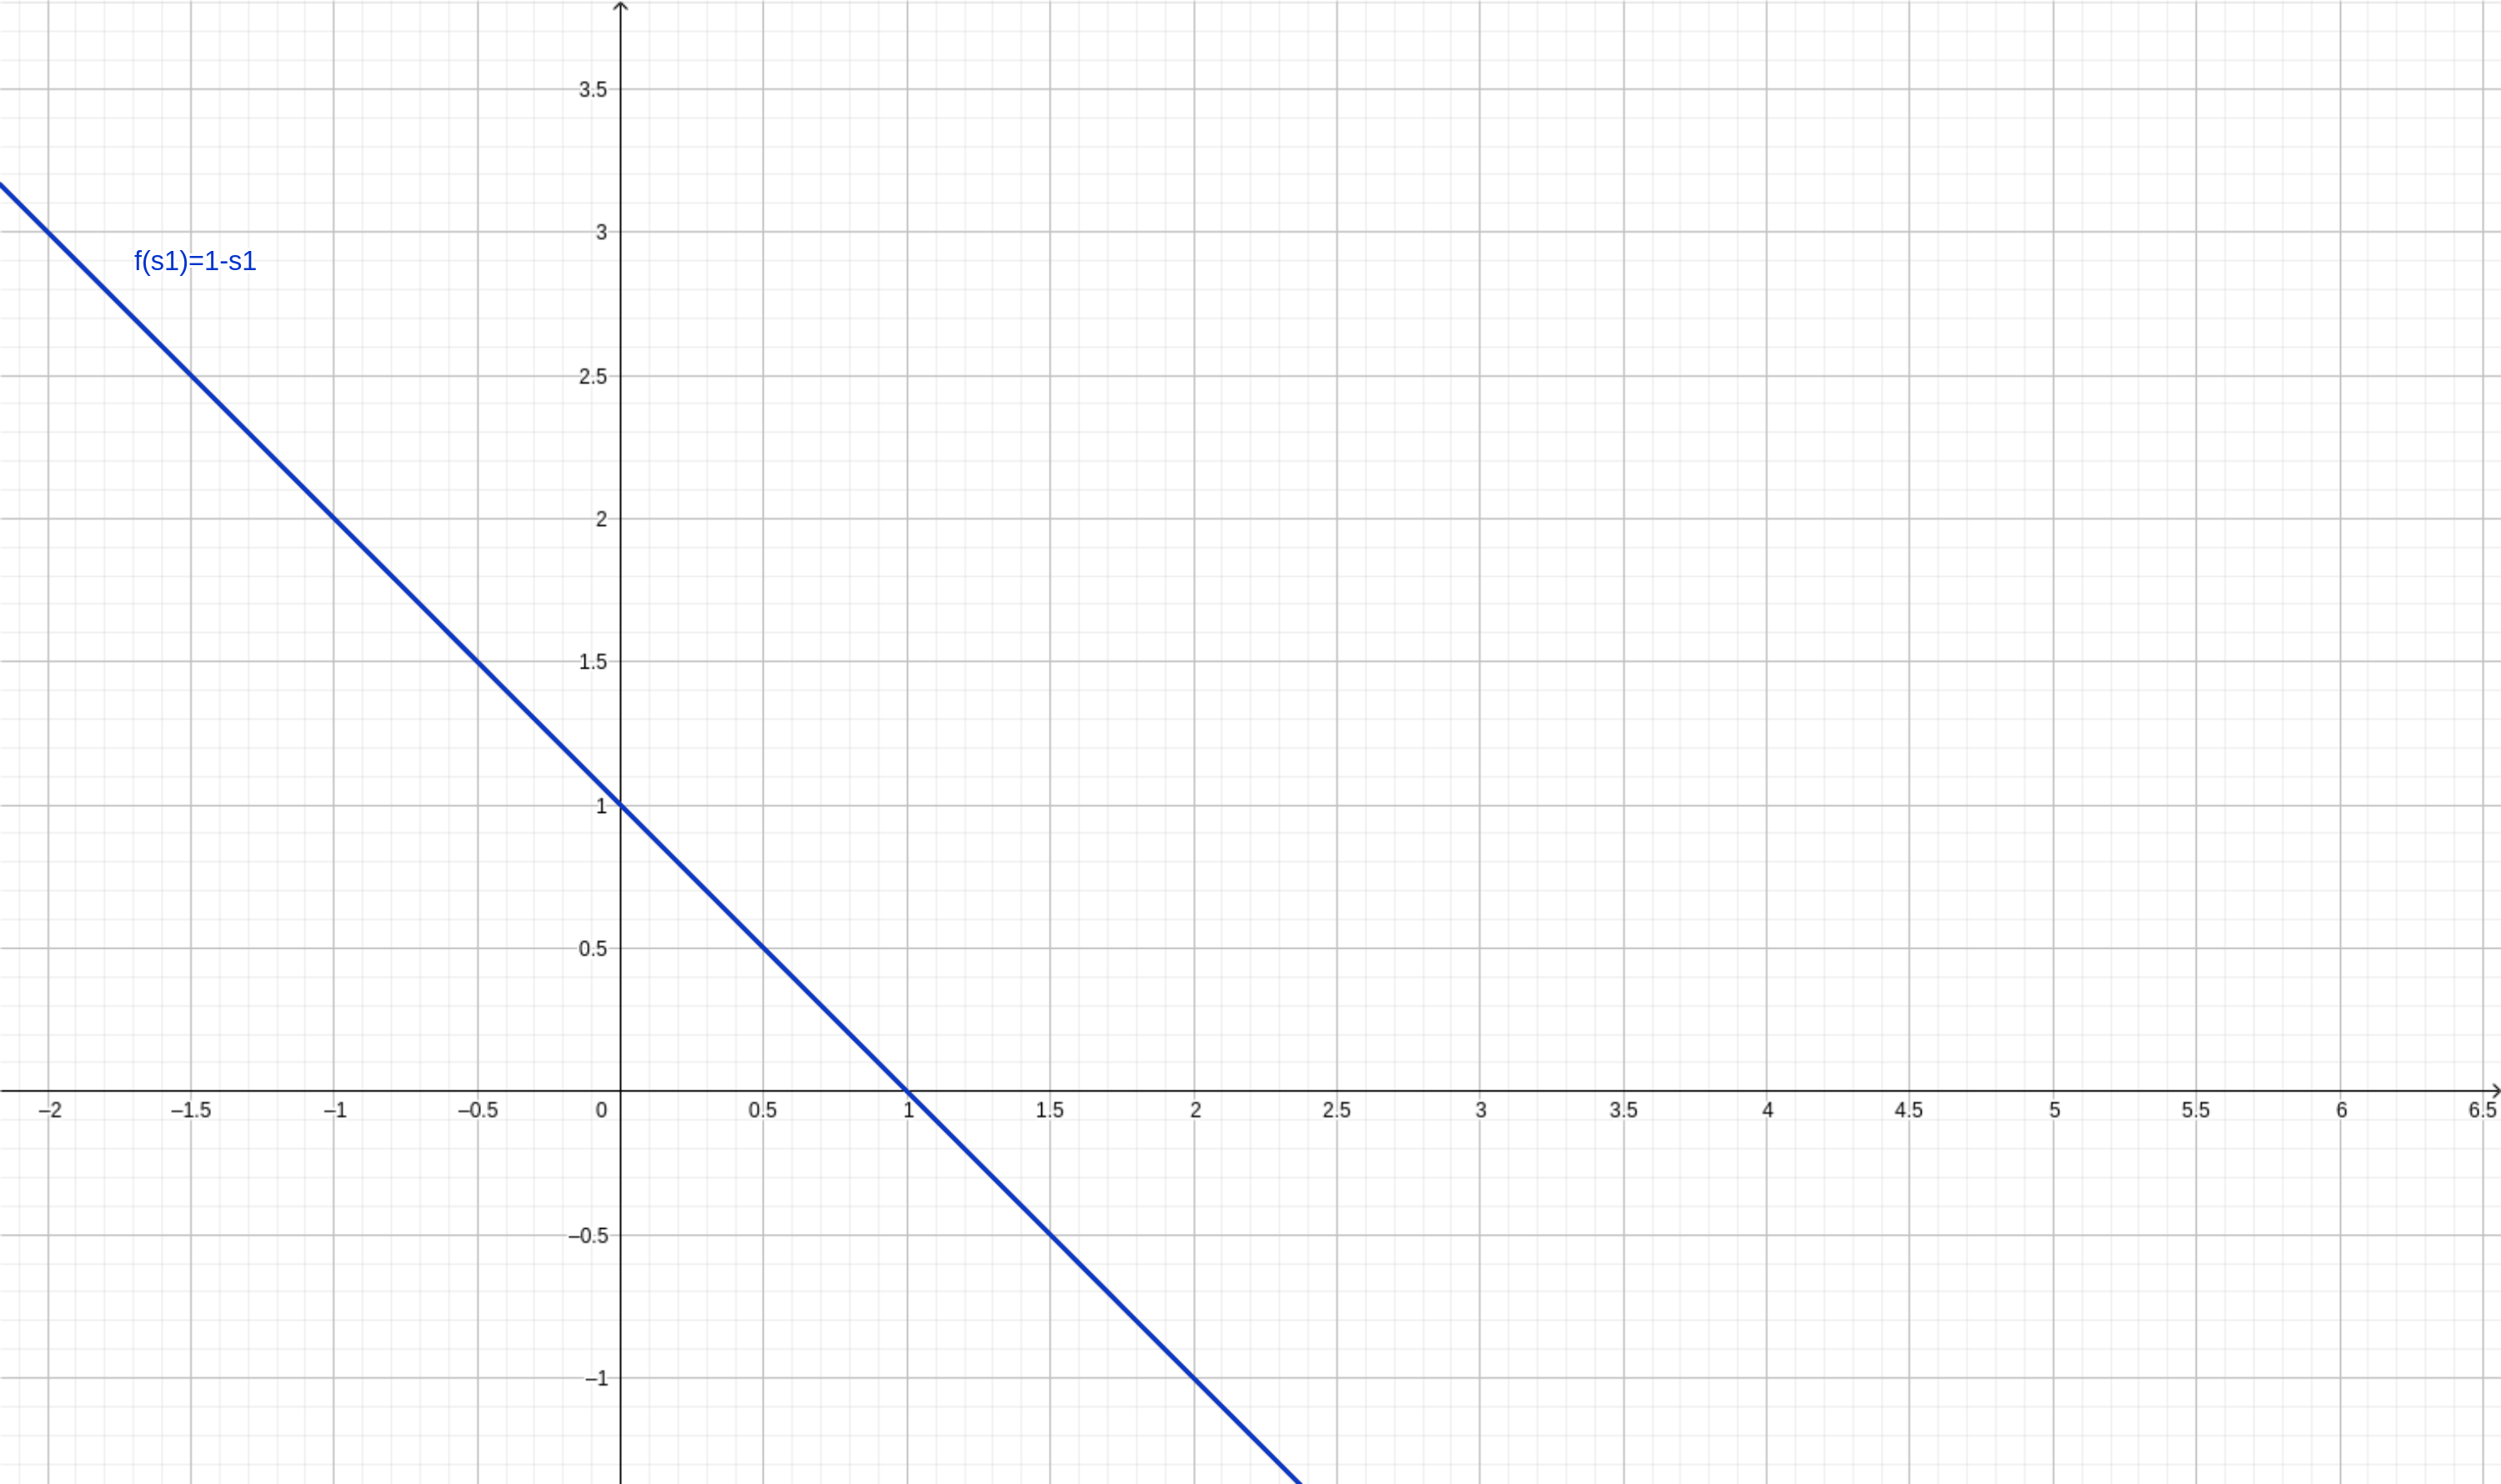
\includegraphics[width=0.90\linewidth]{./image/equazioneretta.png}
	\caption{Rappresentazione della retta passante per $S_0=0$}
\end{figure}
\item Il medesimo ragionamento vale per le rette passanti per $S_1$ e $S_2$.

\begin{center}$S_1=0$ e $S_0+S_2=1$\end{center}
l'asse $S_1$ \`e fissato a 0 e $S_0$ e $S_2$ assumono valori tra (0,1).\\\\

\begin{center} $S_2=0$ e $S_1+S_0=1$ \end{center}
l'asse $S_2$ \`e fissato a 0 e $S_0$ e $S_2$ assumono valori tra (0,1).

\item In questo modo l'unione di tutte le rette passanti per gli assi creano la regione accettabile dei valori di P(A).
\end{enumerate}

\noindent Avendo rappresentato il piano si ottiene nei punti di intersezioni fra le tre rette la regione accettabile per P(A). Inoltre \`e possibile, ora, individuare il fascio di rette che tangenti il piano permettono di affermare se una specifica domanda \`e, in base alla sua frequenza, ha difficolt\`a bassa, media, alta per un candidato.
\begin{itemize}
\item Se una domanda ha una difficolt\`a bassa la retta si situa passante per i punti $0<S_2<=1$ (molto vicino a 1) e $(S_0, S_1)<0$ (tendenti a 0);
\item Se una domanda ha una difficolt\`a alta la retta si situa passante per i punti $S_2<=0$ (molto vicino a 0), $S_1<1$ e $S_0<=1$ (tendente a non scartare alcuna risposta);
\item Se una domanda ha una difficolt\`a media la retta si situa nella parte centrale della regione accettabile, passante per i punti $0<=(S_0, S_1, S_2)<=1$.\end{itemize}

\paragraph{Rappresentazione di P(A)}\mbox\\\\

\noindent Vediamo alcuni casi di come le domande possono venire rappresentate sul piano:\\\\
La funzione di partenza \`e:
\begin{center}$F=\frac{1}{3}+\frac{1}{6}S_1+\frac{2}{3}S_2$\end{center}
Va esplicitato $S_1$, i passaggi utili da fare sono i seguenti:\\\\
$\frac{-1}{6}S_1=\frac{1}{3}+\frac{2}{3}S_2-F$ $\rightarrow$ $S_1=-4S_2-2+6F$\\\\
Essendo  che $0<=S_2<=1$ usando $S_1=1$ e $S_2=0$ allora si ottiene che $F=\frac{1}{2}=0.5$\\
\\
Quanto appena calcolato pu\`o venire rappresentato graficamente impiegando la retta $S_1=1-S_2$ (responsabile di definire una porzione del piano in base alle variaibili coinvolte) e mediante la retta $S_1=-4S_2-2+6F$ (che permette di calcolare il fascio di rette tangenti alla prima retta). \\

\begin{figure}[H]
\centering
	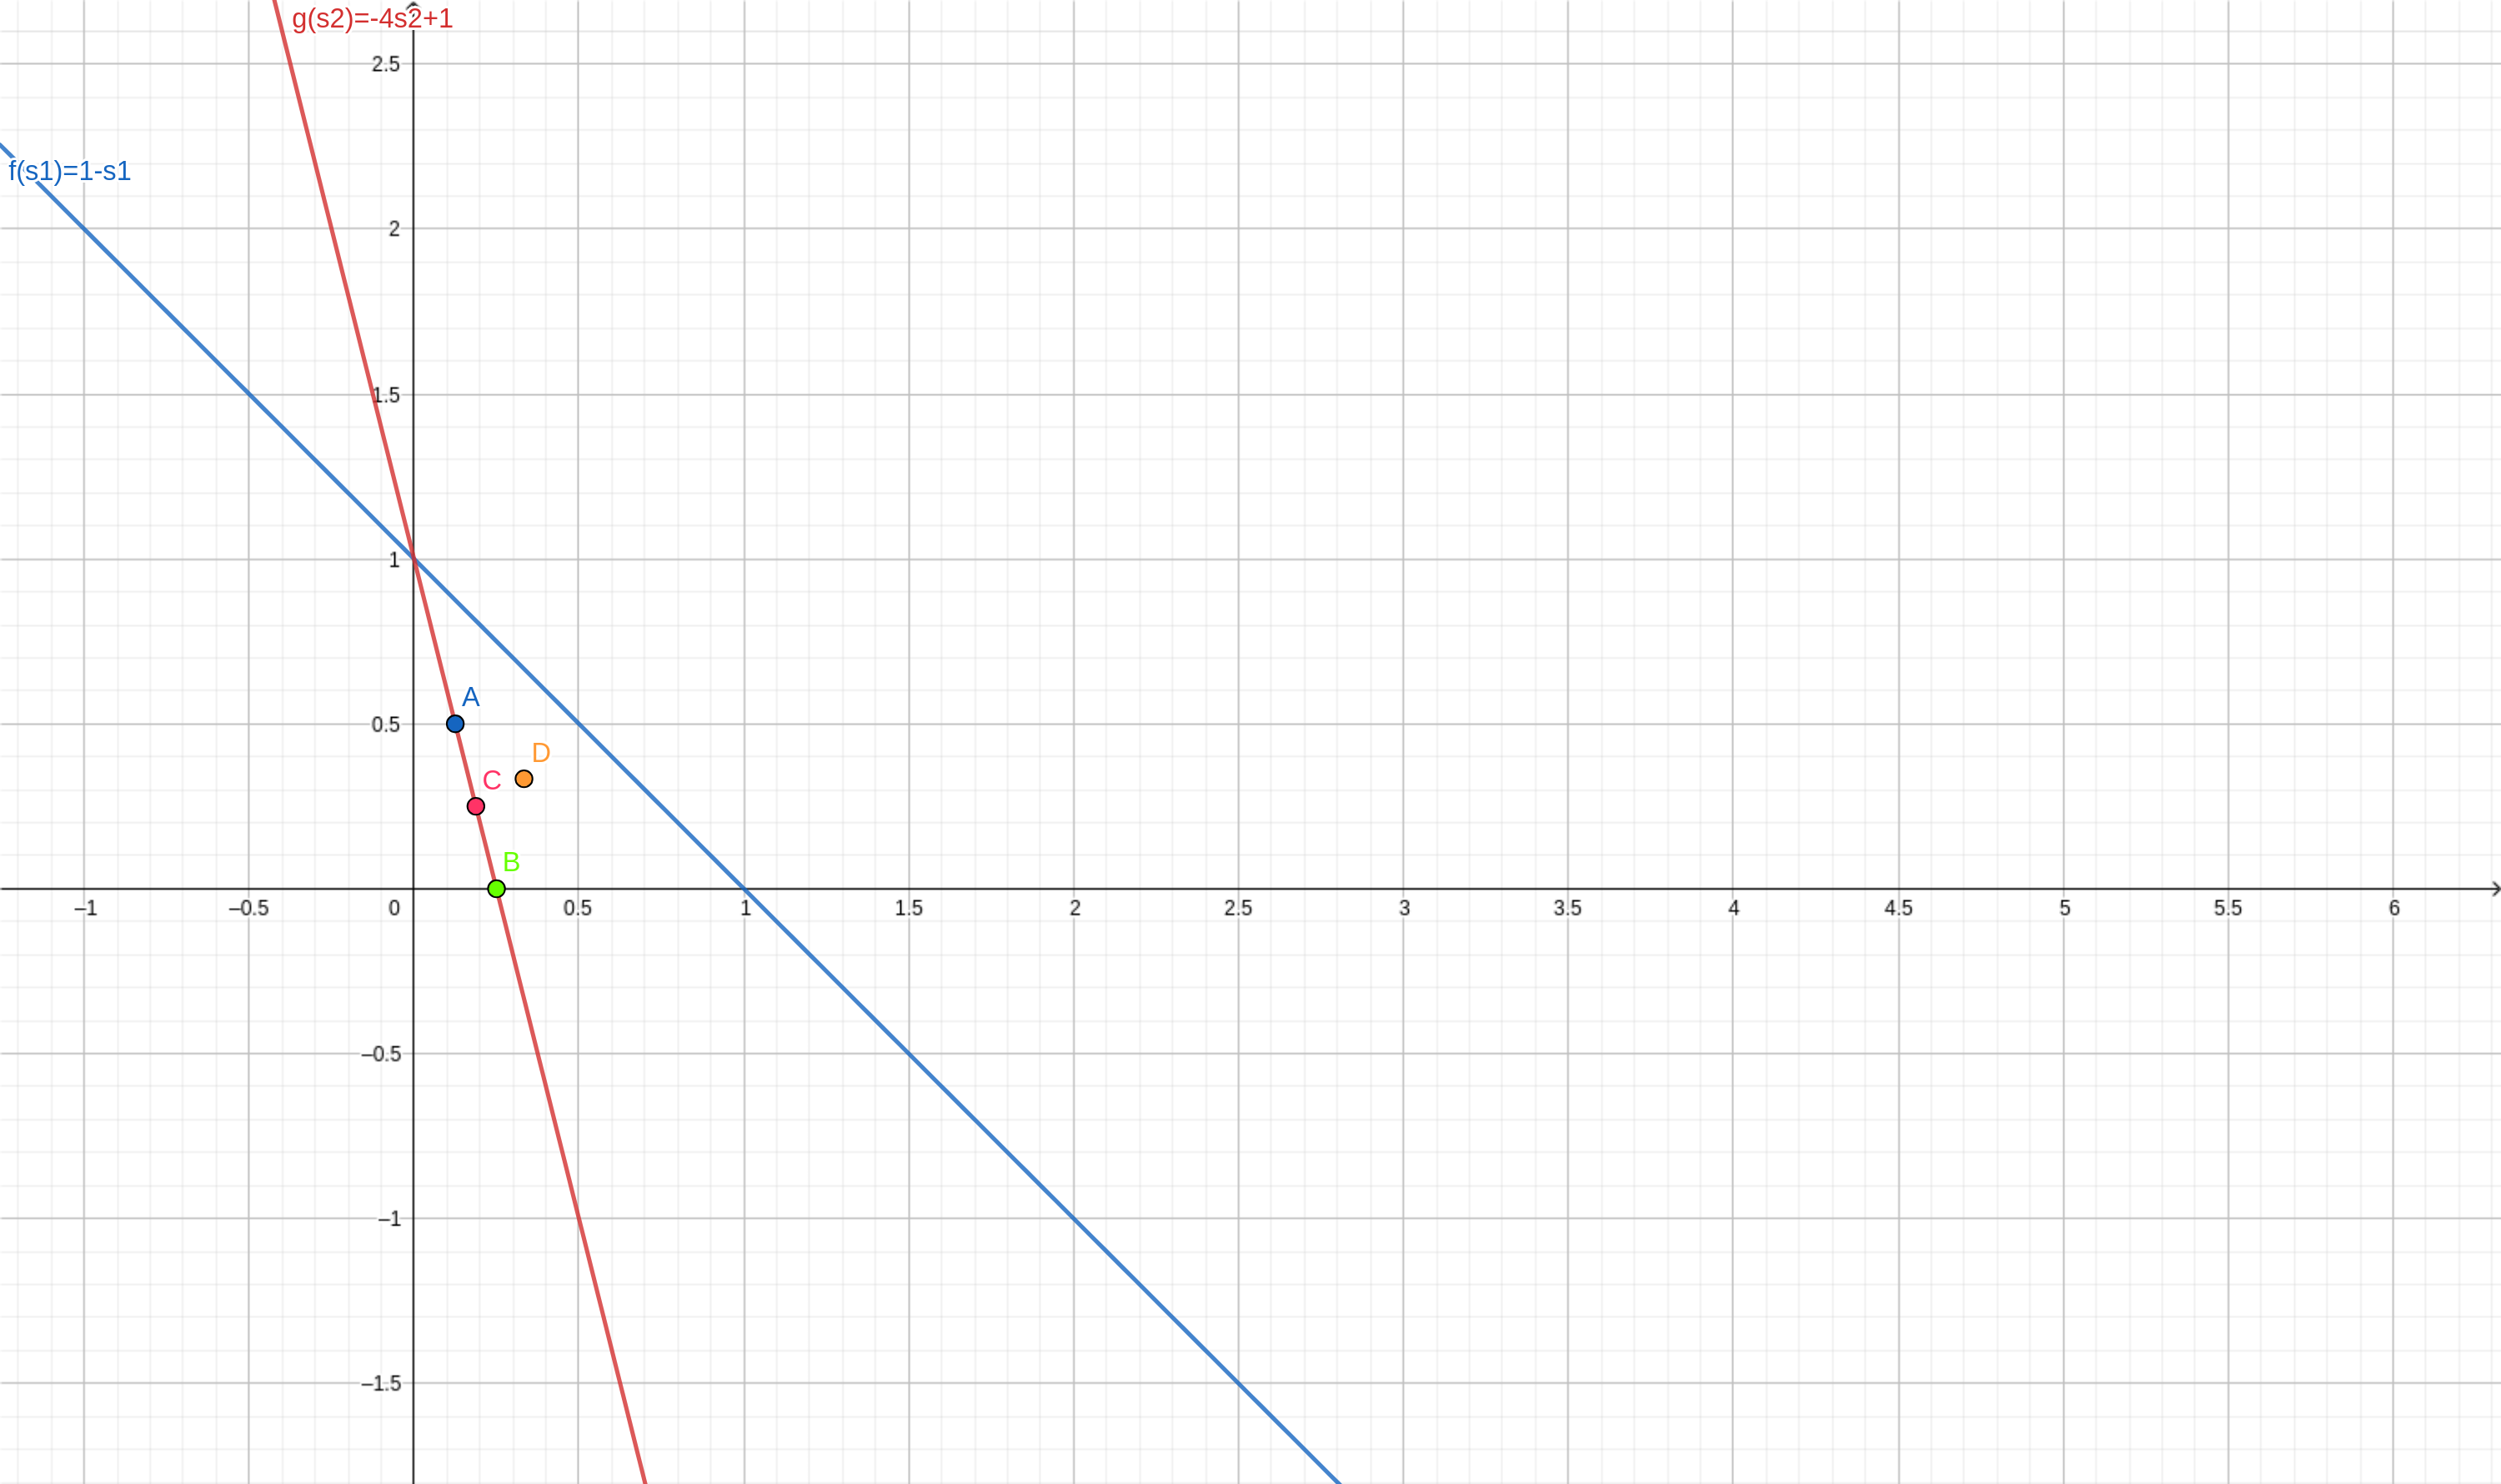
\includegraphics[width=0.90\linewidth]{./image/esempio1.png}
	\caption{Rappresentazione di P(A) per una frequenza 0.5 proiettata su assi $S_0=0$, $S_1$ e $S_2$.}
\end{figure}

\noindent
Nella figura sopra sono rappresentati i seguenti significati:
\begin{itemize}
\item La linea azzurra rappresenta $S_2=1-S_1$;
\item La linea rosa rappresenta la retta tangente $S_1=-4S_2+1$;
\item Punto A (blu): \\
$S_1=0.5=\frac{1}{2}$ \\
$\frac{1}{2}=-4S_2+1$ $\rightarrow$ $4S_2=1-\frac{1}{2}$ $\rightarrow$ $S_2=\frac{1}{8}$ \\
$S_0=1-\frac{1}{2}-\frac{1}{8}=\frac{3}{8}$\\
\\
Ovvero met\`a dei candidati sottoposti alla domanda sa scartare una delle risposte, lo 0.16\% sa dare la risposta corretta e lo 0.36\% non sa scartare alcune delle risposte possibili.
\item Punto B (verde): \\
$S_1=0$\\
$S_2=\frac{1}{4}$\\
$S_0=1-\frac{1}{4}=\frac{3}{4}$\\
\\
Ovvero nessun dei candidati sottoposti alla domanda sa scartare una delle risposte, lo 0.25\% sa dare la risposta corretta e lo 0.75\% non sa scartare alcune delle risposte possibili.
\item Punto C (fucsia): \\
$S_1=\frac{1}{4}$\\
$S_2=\frac{3}{16}$\\
$S_0=1-\frac{1}{4}-\frac{3}{16}=\frac{9}{16}$\\
\\
Ovvero lo 0.25\% dei candidati sottoposti alla domanda sa scartare una delle risposte, lo 0.19\% sa dare la risposta corretta e lo 0.56\% non sa scartare alcune delle risposte possibili.
\item Punto D (arancione): \\
$S_1=\frac{1}{3}$\\
$S_2=\frac{1}{3}$\\
$S_0=1-\frac{1}{3}-\frac{1}{3}=\frac{1}{3}$\\
\\
Osserviamo che il punto in esame fuoriesce dalla regione delimitata dalla retta tangente di frequenza 0.5 ($S_1=-4S_2+1$). Conseguenza diretta data dall'impossibilit\`a di ottenere una probabilit\`a del 50\% sulla domanda con $\frac{1}{3}$ di candidati che sa scartare 2 risposte, $\frac{1}{3}$ che ne sa scartare 1 e $\frac{1}{3}$ nessuna.
\end{itemize}
\noindent
Vediamo ulteriori due esempi che permettono di valutare cosa accade nel piano nel caso di una frequenza:
\begin{enumerate} 
\item Quasi in prossimit\`a di 1;
\item Pari alla soglia minima dell'indovinato.
\end{enumerate}
\noindent

Il grafico \`e il seguente:

\begin{figure}[H]
\centering
	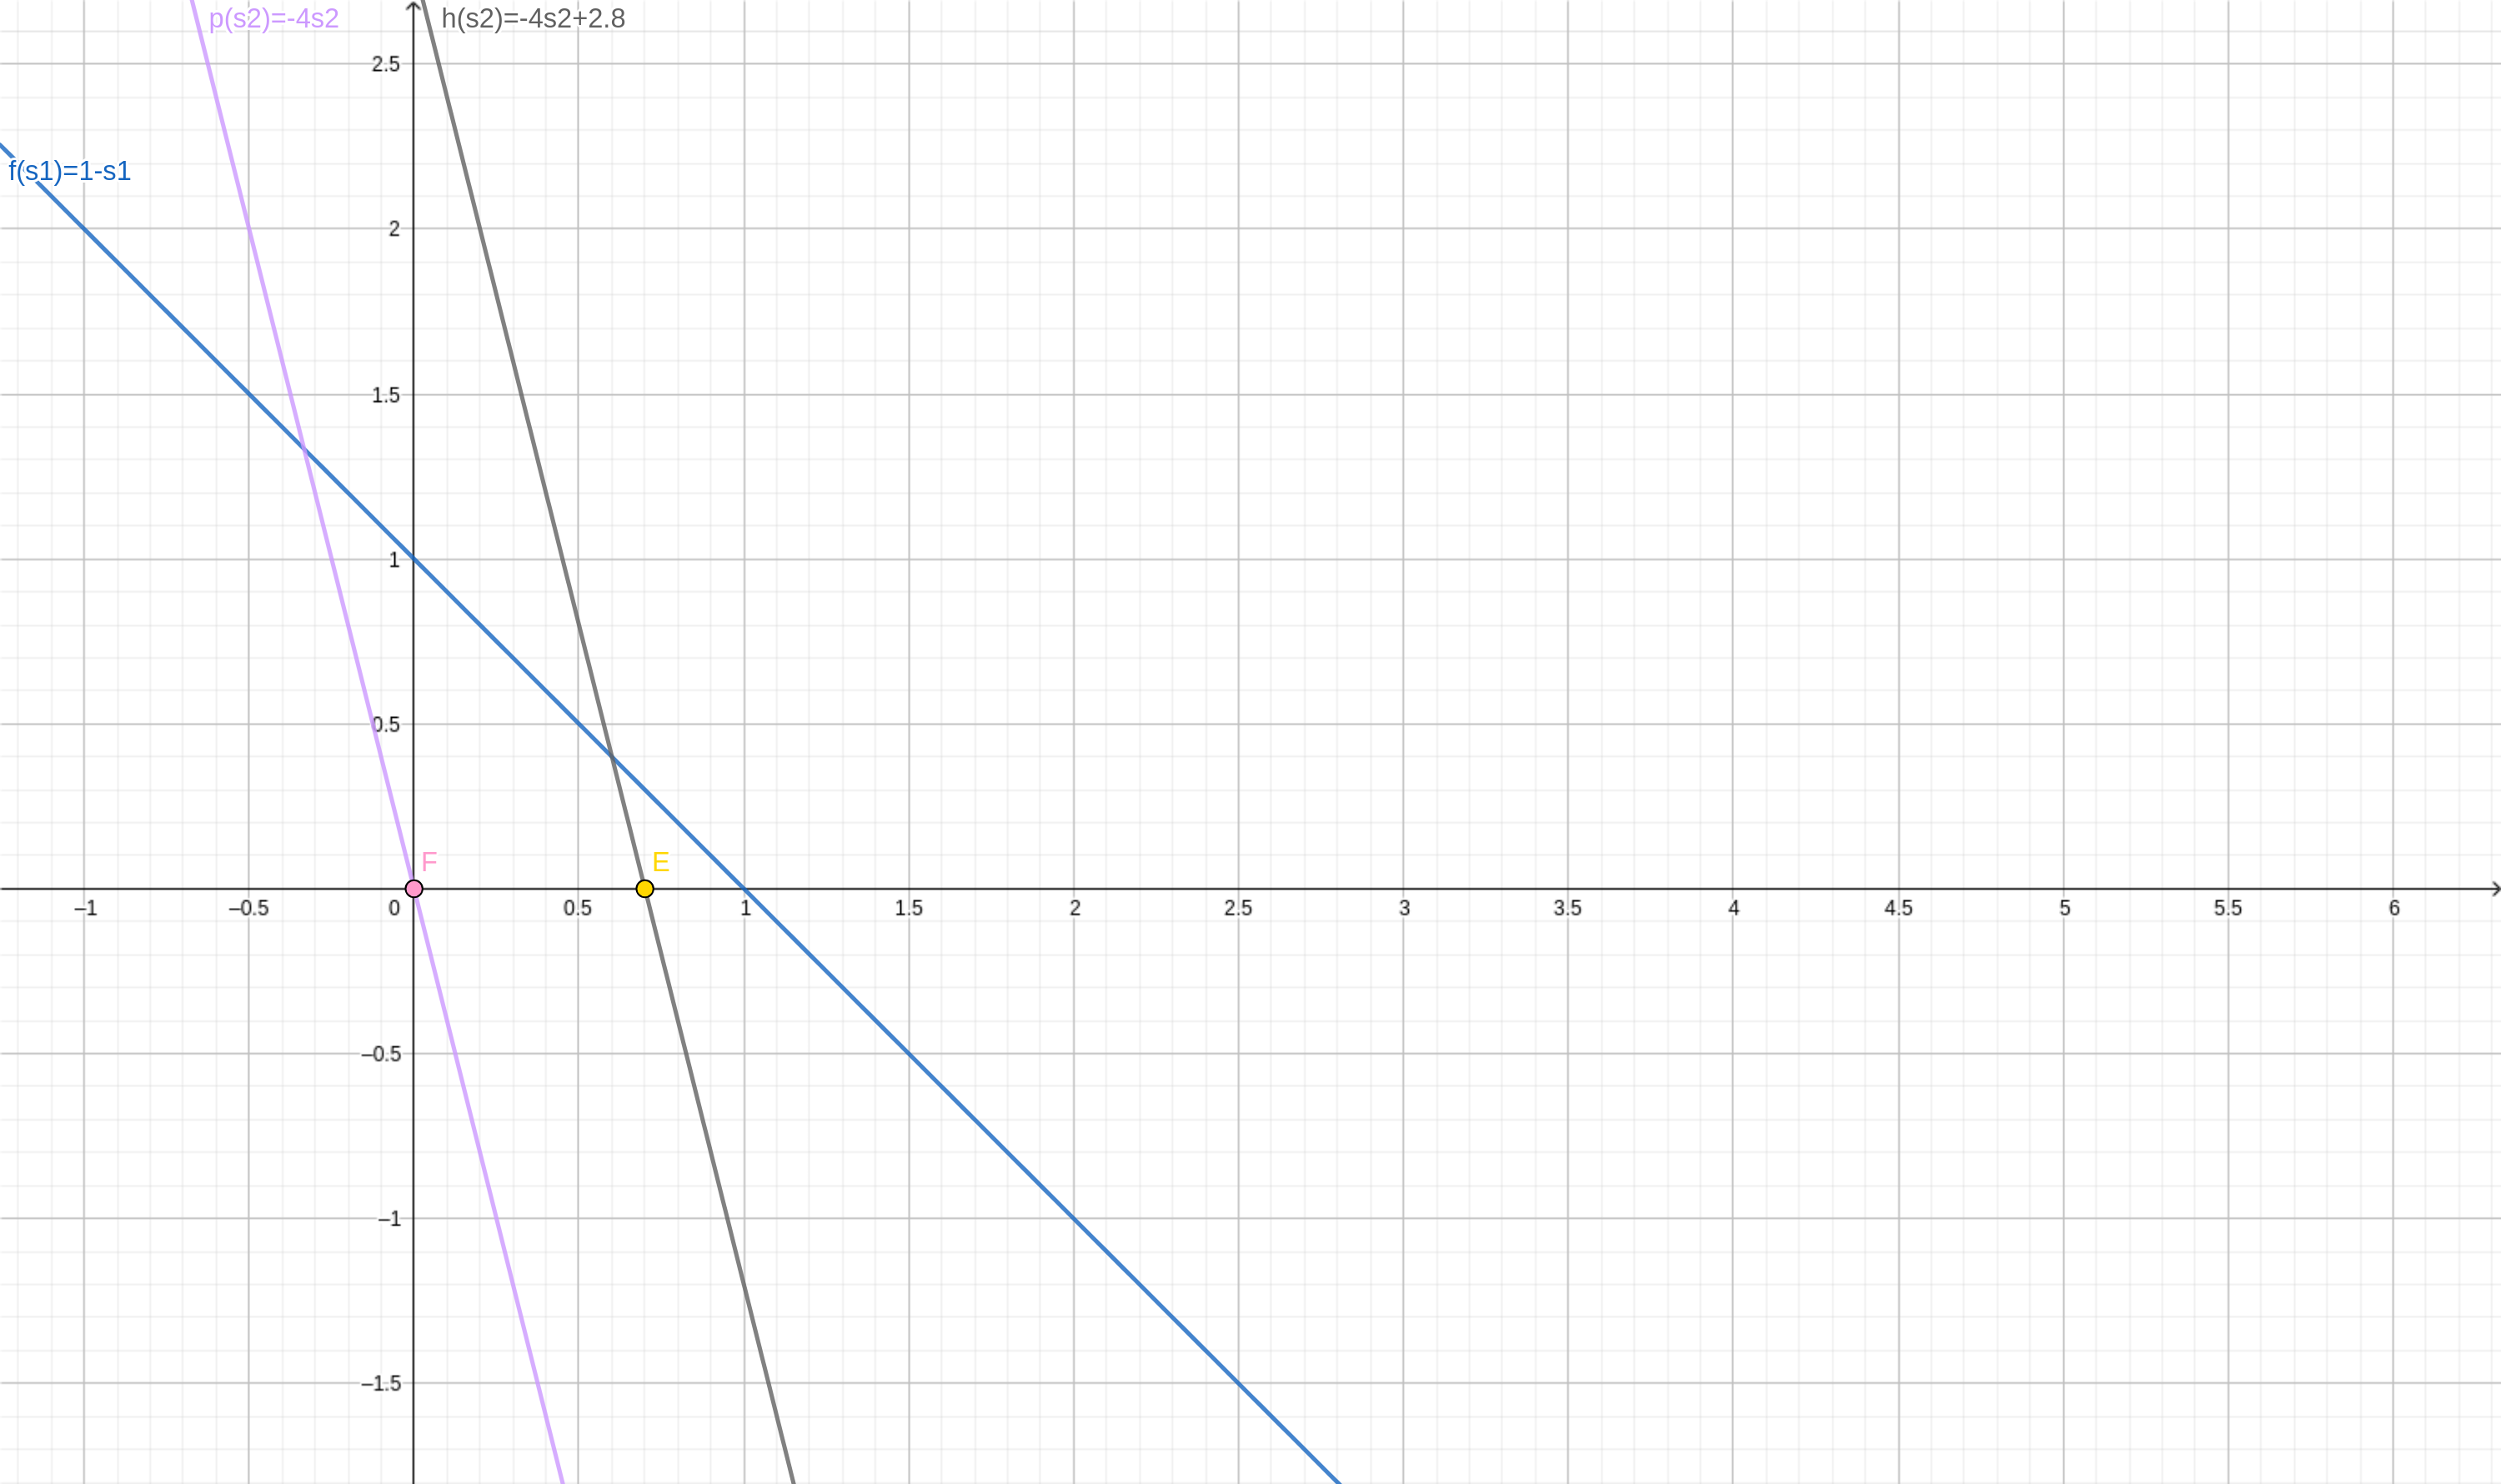
\includegraphics[width=0.90\linewidth]{./image/esempio2.png}
	\caption{Rappresentazione di P(A) per una frequenza 0.33 e 0.8 proiettate su assi $S_0=0$, $S_1$ e $S_2$.}
\end{figure}

\begin{itemize}
\item La linea azzurra mostra la retta tangente con frequenza 0.80\%.
In questa abbiamo calcolato il punto E (giallo):\\
$S_1=0$\\
$S_2=\frac{14}{20}$\\
$S_0=0$\\
\\
Quasi la totalit\`a dei candidati ha la conoscenza per poter scartare tutte le risposte sbagliate e dare la risposta giusta alla domanda.
\item La linea viola mostra la retta tangente con frequenza 0.33\%.
In questa abbiamo calcolato il punto F (rosa):\\
$S_1=0$\\
$S_2=0$\\
$S_0=1$\\
\\ 
Ovvero nessuno dei candidati ha la conoscenza per poter scartare n\`e una n\`e due risposte, percui l'unica possibilit\`a per un candidato di rispondere alla domanda \`e indovinare. \`E evidente come se un candidato non sa la risposta ad una domanda ha una probabilit\`a dello 0.33\% di poter indovinare la risposta corretta.
\end{itemize}


